我们选取的校园场景图片如图1所示。
\begin{figure}[h!]
    \centering
    \includegraphics[width=\textwidth]{imgs/origin.png}
    \caption{原始校园场景图片}
    \label{fig:origin_image}
\end{figure}

\subsubsection{MMDetection 检测结果}
我们利用MMDetection的API工具,检测到的结果如图2所示。

\begin{figure}[h!]
    \centering
    \includegraphics[width=\textwidth]{imgs/mmdetection.png}
    \caption{FCOS 检测结果示意图}
    \label{fig:fcos_result}
\end{figure}


\subsubsection{YOLOv8 检测结果}
我们利用MMDetection的API工具,检测到的结果如图3所示。

\begin{figure}[h!]
    \centering
    \includegraphics[width=\textwidth]{imgs/yolo.png}
    \caption{YOLOv8 检测结果示意图}
    \label{fig:yolov8_result}
\end{figure}

\subsubsection{Faster R-CNN 检测结果}
由于此API没有可视化较好的工具,
因此选择一张样例图片,这是上述场景图片的第四张。
输出检测出的bbox坐标,结果如图4所示。

\begin{figure}[h!]
    \centering
    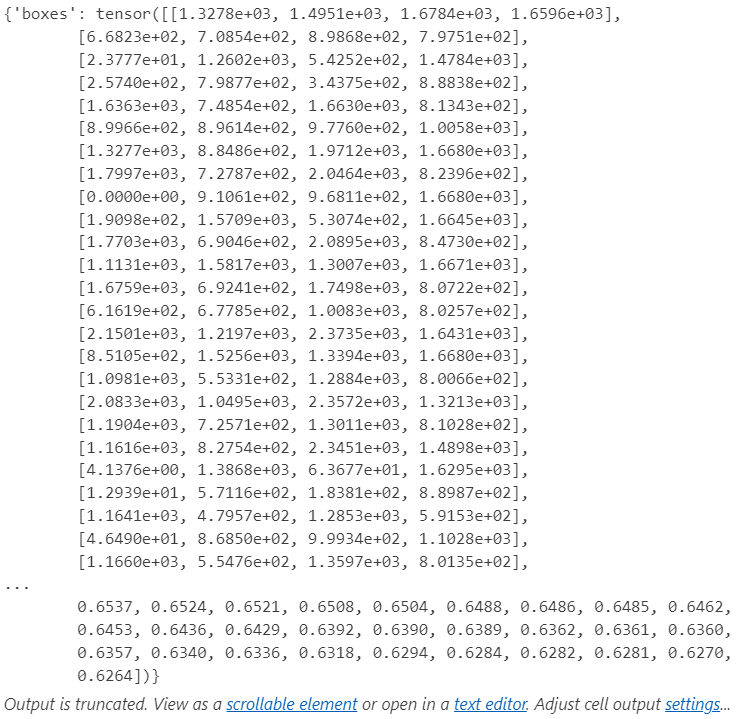
\includegraphics[width=\textwidth]{imgs/fast_res.png}
    \caption{Faster R-CNN 检测结果示意图}
    \label{fig:fasterrcnn_result}
\end{figure}


